% \section{Evaluation: Recasting Type Errors as Runtime Errors}
\section{Evaluation}
\label{sec:evaluation}

We have implemented a prototype of our search procedure and trace
visualization for a purely functional subset of \ocaml\ --- with
polymorphic types and records, but no modules, objects, or polymorphic
variants --- in a tool called \nanomaly.
%
We treat explicit type signatures, \eg @(x : int)@, as
primitive operations that narrow the type of the wrapped value.
%
In our implementation we instantiated \gensym\ with a simple random
generation of values, which we will show suffices for the majority of
type errors.

\paragraph{Evaluation Goals}
%
There are four questions we seek to answer with our evaluation:
%
\begin{enumerate}
\item \emphbf{Witness Coverage} (\S~\ref{sec:eval:witness-coverage},~\ref{sec:how-safe})
      How many ill-typed programs \emph{admit} witnesses?
\item \emphbf{Witness Complexity} (\S~\ref{sec:trace-complexity})
      How \emph{complex} are the traces produced by the witnesses?
\item \emphbf{Witness Utility} (\S~\ref{sec:advantage-traces},~\ref{sec:user-study})
      How \emph{helpful} %(qualitatively and quantitatively)
      are the witnesses in debugging type errors?
\item \emphbf{Witness-based Blame} (\S~\ref{sec:locating})
      Can witnesses be used to \emph{locate} the source
      of an error?
\end{enumerate}

In the sequel we present our experimental methodology (\S~\ref{sec:methodology})
and then answer the above questions.
%
However, for the impatient reader, we first summarize our main results:

\paragraph{1. Most Type Errors Admit Witnesses}
Our prime result is that the vast majority of static type errors, around
85\%, do in fact admit a dynamic witness.
%
Further, \toolname efficiently synthesizes witnesses with its randomized search;
it can synthesize a witness for over 75\% of programs in under one second, \ie
fast enough for interactive use. %to be integrated into the edit-compile-debug cycle.
%

\paragraph{2. Jump-Compressed Traces Are Small}
We find that our jump-compression heuristic effectively abstracts the
pedestrian details of computation, compressing the median trace with
14--15 single-step reductions to only 4 jumps.
%
Over 80\% of programs have a jump-compressed trace with at most 10
jumps, providing a bird's-eye view from which we can launch a more
in-depth investigation.

\paragraph{3. Witnesses Help Novices}
A witness should also help programmers \emph{understand} and
\emph{fix} type errors.
%
We use a set of ill-typed student programs to show that \toolname's
witnesses effectively demonstrate the runtime error that the type
system prevented.
%
Furthermore, we find, in a study of undergraduate students, that
\toolname's witnesses lead to more accurate diagnoses and fixes of type
errors than \ocaml's type error messages.

\paragraph{4. Witnesses Assign Blame}
Finally, we present a simple heuristic that allows us to use witnesses
to \emph{automatically} assign blame for type errors.
%
We treat the values inside the stuck term as \emph{sources} of typing
constraints and the stuck term itself as a \emph{sink}, producing
a slice of the program that likely contains the error.
%
Using this heuristic, \toolname's witness are competitive with the
state-of-the-art localization tools \mycroft and \sherrloc.

\subsection{Methodology}
\label{sec:methodology}
We answer the first two questions on two sets of ill-typed programs,
\ie\ programs that were rejected by the \ocaml\ compiler because of a
type error.
%
The first dataset comes from the Spring 2014 undergraduate Programming
Languages (CSE 130) course at UC San Diego.
%
We recorded each interaction with the \ocaml\ top-level system over the
course of the first three assignments (IRB
% \# hidden for blind review),
\#140608),
from which we extracted \ucsdsize\ distinct, ill-typed \ocaml\ programs
from a cohort of 46 students..
%
The second dataset --- widely used in the literature --- comes from a
graduate-level course at the University of Washington~\cite{Lerner2006-pj},
from which we extracted 284 ill-typed programs.
%
Both datasets contain relatively small programs, the largest being 348
SLoC; however, they demonstrate a variety of functional programming
idioms including (tail) recursive functions, higher-order functions,
polymorphic and algebraic data types. % and expression evaluators.

We answer the third question in two steps.
%
First, we present a qualitative evaluation of \toolname's traces on a
selection of programs drawn from the UCSD dataset.
%
Second, we present a quantitative user study of students in the
University of Virginia's Spring 2016 undergraduate Programming Languages
(CS 4501) course.
%
As part of an exam, we presented the students with ill-typed \ocaml\
programs and asked them to
%
(1) \emph{explain} the type error, and
%
(2) \emph{fix} the type error (IRB \#2014009900).
%
For each problem the students were given the ill-typed program and
either \ocaml's error message or \toolname's jump-compressed trace.

We answer the last question on a subset of the \ucsdbench dataset.
%
For each ill-typed program in a student's interaction trace, we identify
the student's \emph{fix} by searching for the first type-correct program
that follows it in the trace.
%
We then use an expression-level \emph{diff}~\cite{Lempsink2009-xf} to
determine which sub-expressions changed between the ill-typed program
and the student's fix, and treat those expressions as the source of the
type error.

\subsection{Witness Coverage}
\label{sec:eval:witness-coverage}
%
We ran our search algorithm on each program for 1,000 iterations, with
the entry point set to the function that \ocaml\ had identified as
containing a type error.
%
Due to the possibility of non-termination we set a timeout of one minute
total per program.
%
% Due to the possibility of non-termination we set a limit on the number
% of reductions to perform, increasing in 500-step increments from 500
% steps to 3,000 steps total.
%
We also added a na{\"\i}ve check for infinite recursion; at each recursive
function call we check whether the new arguments are identical to the
current arguments.
%
If so, the function cannot possibly terminate and we report an error.
%
While not a \emph{type error}, infinite recursion is still a clear bug
in the program, and thus valuable feedback for the user.

\begin{figure}[t]
% \centerline{
% \begin{minipage}{1.2\textwidth}
\centering
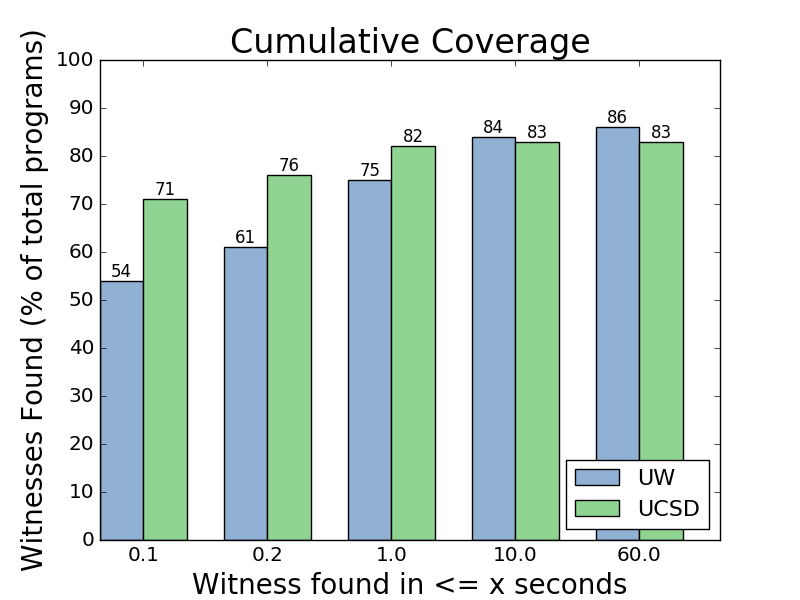
\includegraphics[width=0.7\linewidth]{coverage.png}
% \end{minipage}
% \begin{minipage}{\linewidth}
% 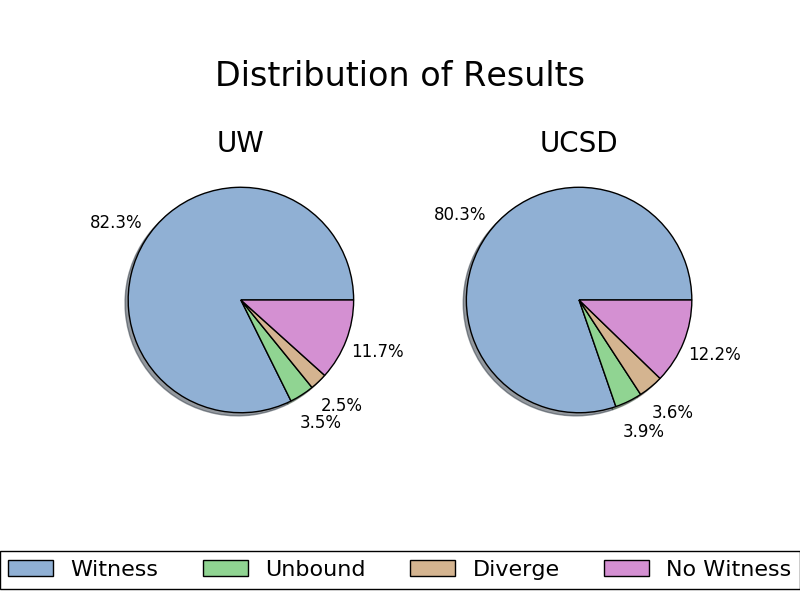
\includegraphics[width=0.6\linewidth]{distrib.png}
% \end{minipage}
% }
% \vspace{3ex}
\caption{Results of our coverage testing. Our random search successfully
  finds witnesses for 76--82\% of the programs in under one second,
  improving to 84--85\% in under 10 seconds. }
\label{fig:results-witness}
\end{figure}
\begin{figure}[t]
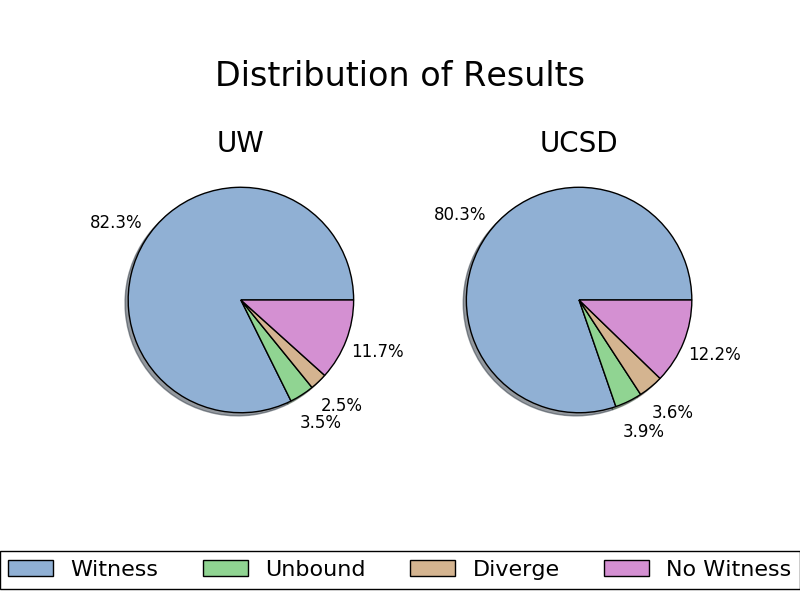
\includegraphics[width=0.7\linewidth]{distrib.png}
\caption{Distribution of test outcomes. In both datasets we detect
  actual type errors at least 75\% of the time, unbound variables or
  constructors 4--5\% of the time, and diverging loops 3\% of the
  time. For the remaining 13--16\% of the programs we are unable to
  provide any useful feedback. }
\label{fig:results-distrib}
\end{figure}


\paragraph{Results}
\label{sec:results-witness}
The results of our experiments are summarized in
Figures~\ref{fig:results-witness}~and~\ref{fig:results-distrib}.
%
In both datasets our tool was able to find a witness for over 75\% of the
programs in under one second, \ie\ fast enough to be integrated as a
compile-time check. If we extend our tolerance to a 10 second timeout,
we reach 84--85\% coverage, and if we allow a 60 second search,
we hit a maximum of 84--87\% coverage.
%
Interestingly, while the vast majority of witnesses corresponded to a
type-error, as expected, 4--5\% triggered an unbound variable error (even
though \ocaml\ reported a type error) and 3\% triggered an infinite
recursion error.
%
For the remaining 13--16\% of programs we were unable to provide any useful
feedback as they either completed 1,000 tests successfully, or timed out
after one minute.
%
% XX programs were deemed safe and XX timed out even at 3,000 steps, \ie
% we could not provide any useful feedback for XX\% of the total programs.
%
While a more advanced search procedure, \eg\ dynamic-symbolic execution,
could likely uncover more errors, our experiments suggest that
type errors are coarse enough (or that novice programs are \emph{simple}
enough) that these techniques are not necessary.

\subsection{How safe are the ``safe'' programs?}
\label{sec:how-safe}

An immediate question arises regarding the 13--16\% of programs for
which we could not synthesize a witness:
%
are they \emph{actually} safe (\ie is the type system being too conservative),
%
or did \toolname simply fail to find a witness?
%
% \ES{Need better organization for the groupings of programs, maybe a pie chart to guide us?}

To answer this question, we investigated the 720 \ucsdbench programs for
which we failed to find a witness.
%
We used a combination of automatic and manual coding to categorize these
programs into four classes.
%
The first class is easily detected by \toolname itself, and thus admits
a precise count.
%
This left us with 473 programs that required manual coding; we selected
a random sample of 50 programs to investigate, and will report results
based on that sample.
%
Figure~\ref{fig:no-witness} summarizes the results of our investigation ---
we note the classes that were based on the random sample with a ``*''.


\begin{figure}[t]
%\centering
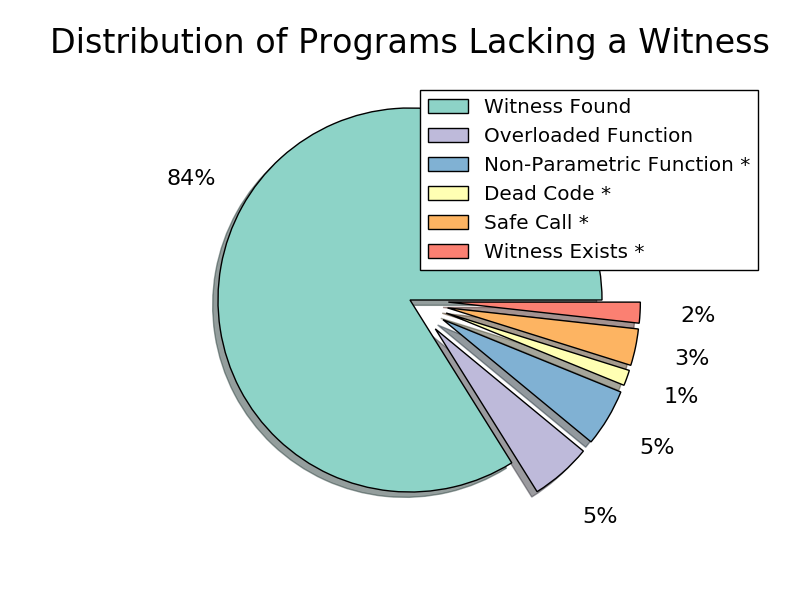
\includegraphics[width=0.7\linewidth]{distrib_ext.png}
\vspace{-0.75cm}
\caption{Results of our investigation into programs where \toolname
  did not produce a witness. A ``*'' denotes that the percentage is an
  estimate based on a random sampling of 50 programs.}
\label{fig:no-witness}
\end{figure}

\paragraph{Ad-Hoc Polymorphism}
%
We found that for 5\% programs \toolname got stuck when it tried to
compare two holes.
%
\ocaml provides polymorphic equality and comparison operators,
overloading them for each type.
%
While convenient to use, they pose a challenge for \toolname's
combination of execution and inference.
%
For example, consider the \hbox{@n <= 0@} test in our @fac@ example.
%
The @<=@ operator is polymorphic, but in this case we can make progress because
the literal @0@ is not.
%
Suppose, however, we parameterized @fac@ by a lower bound, \eg
%
\begin{code}
  let rec fac n m =
    if n <= m then
      true
    else
      n * fac (n - 1) m
\end{code}
%
When given @fac@, \toolname will generate two fresh holes
$\nu_1[\alpha_1]$ and $\nu_2[\alpha_2]$ and proceed directly into the
@n < m@ comparison.
%
We cannot (yet) instantiate either hole because we have no constraints
on the $\alpha$s (we know they must be equal, but nothing else), and
furthermore we do not know what constraints we may encounter later on in
the program.
%
Thus, we cannot perform the comparison and proceed, and must give up our
search for a witness, even though one obviously exists, any pair of |n|
and |m| such that |n <= m| is false.

Extending \toolname with support for symbolic execution would alleviate
this issue, as we could then begin symbolically executing the program
until we learn how to instantiate |n| and |m|.
%
Alternatively, we could \emph{speculatively} instantiate both |n| and
|m| with some arbitrary type, and proceed with execution until we
discover a type error.
%
This speculative instantiation is, of course, unsound; we would have to
take care to avoid reporting frivolous type errors that were caused by
such instantiations.
%
We would need to track which holes were instantiated speculatively 
to distinguish type errors that would have happened regardless, as
in @fac@, from type errors that were caused by our instantiation.

Further, suppose that our speculative instantiation induces a frivolous
type error.
%
For example, suppose we are given
%
\begin{code}
  let bad x y =
    if x < y then
      x *. y
    else
      0.0
\end{code}
%
and choose to (speculatively) instantiate @x@ and @y@ as @int@s and proceed
down the ``true'' branch.
%
We will quickly discover this was the wrong choice, as they are immediately
narrowed to @float@s.
%
We must now backtrack and try a different instantiation, but we no
longer need to choose one at random.
%
Since our instantiation was speculative, and @x@ and @y@
% WRW thinks "morally" is too informal for this venue. 
were \emph{originally} hole, we can treat the @*.@ operator as a normal
narrowing point with two holes.
%
This tells us that the \emph{correct} instantiation was in fact @float@,
and we can then proceed as normal from the backtracking point with a
concrete choice of @float@s.
%
Thus, it appears that speculative instantiation of holes may be a
useful, lightweight alternative to symbolic execution for our purposes.

% \paragraph{} \hspace{0ex} \\
% The remaining 473 programs for which we could not produce a witness did
% not admit such an automatic diagnosis, so we selected a random sample of
% 50 programs and manually searched for a witness.
% %
% We categorized the programs into three groups.


\paragraph{Non-Parametric Function Type *}
%
5\% of programs lack a witness in our semantics due to our
non-parametric $\tfun$ type for functions.
%
Recall that our goal is to expose the runtime errors that would have
been prevented by the type systems.
%
At runtime, it is always safe to call a function, thus we give functions
a simple type $\tfun$ that says they may be applied, but says nothing
about their inputs or outputs.
%
But consider the following @clone@ function, which is supposed to
produce a list containing @n@ copies of the input @x@.
%
% Seven programs violated the \emph{occurs check} with cyclic typing
% constraints like @'a = 'a list@, for example the following @clone@
% function.
%
\begin{code}
  let rec clone x n =
    if n > 0 then
      clone [x] (n - 1)
    else
      []
\end{code}
%
Unfortunately, the student instead constructs an @n@-level nested list
containing a single @x@.
%
The \ocaml compiler rejects this program because the recursive call to
@clone@ induces a cyclic typing constraint @'a = 'a list@, capturing the
fact that each call increases the nesting of the list.
%
\toolname fails to catch this because we do not track the types of the
inputs to @clone@.

We note, however, that @clone@ cannot go wrong; it is perfectly safe to
repeatedly enclose a list inside another (disregarding the fact that the
nested list is never returned).
%
Still, such a function would be very difficult to \emph{call} safely, as
the programmer would have to reason about the dependency between the
input @n@ and the nesting of the output list, which cannot be expressed
in \ocaml's type system.

Thus, it is not particularly satisfying that \toolname fails to produce
a witness here; a possible solution could be to track the types of the
inputs, and demonstrate to the user how they change between recursive
calls.
%
This would require maintaining a typing environment of variables in
addition to the environments we maintain for holes.
%
We would have to modify the rule $\reappgood$ from
Figure~\ref{fig:operational} to additionally $\forcesym$ the function's
type against the concrete inputs.
%
However, we would want to ensure that this $\forcesym$ cannot fail ---
it is preferable to report a stuck term as that provides a fuller view
of the error.
%
Rather, we would note which evaluation steps induced incompatible
type refinements, and if a traditional witness cannot be found, we could
then report a trace expanded to show precisely these steps.
%
This represents only a modest extension to our semantics, and would be
interesting to explore further.

\paragraph{Dead Code and ``Safe'' Function Calls *}
%
4\% of programs contained type errors that were unreachable, either
because they were dead code, or because the student called the function
with inputs that could not trigger the error.


1\% contained type errors that were unreachable by any inputs, often due
to overlapping patterns in a @match@ expression.
%
% While technically safe, dead code is generally considered a ``code
% smell''; students would likely benefit from a warning in this case.
% \ES{Wes says this is too informal, source the claim}
%
While technically safe, dead code is generally considered a maintenance
risk, as the programmer may not realize that it is dead~\cite{Wheeler2014-fg}
or may accidentally bring it back to life~\cite{Seven2014-gf}.
%
Thus, a warning like that provided by \ocaml's pattern exhaustiveness
checker would be helpful.

%\paragraph{Bad Function Calls}
A further 3\% included a function call where the
student supplied ill-typed inputs, but the path induced
by the call did not contain an error.
%
Consider the following |assoc| function, which
looks up a key in an \emph{association list}, returning a default if
it cannot be found.
%
\begin{code}
  let rec assoc (d, k, l) = match l with
    | (ki, vi)::tl ->
       if ki = k then
         vi
       else
         assoc (d, k, tl)
    | _ -> d

  let _ = assoc ([], 123, [(123, "sad"); (321, "happy")])
\end{code}
%
The student's definition of |assoc| is correct, but \ocaml rejects their
subsequent call because the default value |[]| is incompatible with the
|string| values in the list.
%
In this particular call the key |123| is in the list, so the default
will not be used (even if it were, there would not be an error) and
\ocaml's complaint is moot.
%
Of course, \ocaml cannot be expected to know that this particular call
is safe, its type system is not sophisticated enough to express the
necessary conditions.
%
% \ES{TODO: add some comment about using dependent types, though this particular example would be quite bizarre to encode in DT..}

% We note that many of the programs in this category appear to come from
% interactions with the \ocaml top-level, \ie the student defined a
% function and is now experimenting with it.
% %
% These calls are thus particularly harmless, indeed they may even be
% \emph{beneficial}, as the student may next try looking up a key that
% \emph{does not} exist, and realize that the returned values are
% incompatible.
% \ES{Wes doesn't like this, sounds like punting on the issue}

\paragraph{Witness Exists *}
%
We found that only 2\% of programs admit a witness that \toolname
was unable to discover.
%
Slightly over half involved synthesizing a \emph{pair} of
specially-crafted inputs that would result in the function returning
values of incompatible types.
%
The rest required synthesizing an input that would trigger a
particular path through the program, and would likely have been caught
by symbolic execution.

\paragraph{Summary}
%
Our investigation suggests that the vast majority of programs
for which we fail to find a witness do not, in fact, admit a
witness.
%
% Overall, it appears that our random instantiation of holes is well-suited
% to finding type errors in student programs.
These programs were generally cases where \ocaml's type system was
overly conservative.
%
Of course, the conservatism is somewhat justified as each case pointed
to code that would be difficult to use or maintain;
%
it would be interesting to investigate how demonstrate these issues in an
intuitive manner.

% \begin{enumerate}
% \item 7 infinite type. program doesn't go wrong, but could search for
%   context that would go wrong
% \item 15 monomorphic functions. recall we abstract a function's type as
%   $\tfun$ rather than $\alpha \to \beta$. (may also admit witness by
%   searching for context?)
% \item 6 dead code. type error occurs in unreachable code, ``deficiency''
%   of the type system.
% \item 14 bad call. function is well-typed, student calls makes ill-typed
%   call, but no error triggered. nothing to be done, as we do not control
%   call-site.
% \end{enumerate}

%%% Local Variables:
%%% mode: latex
%%% TeX-master: "main"
%%% End:



\subsection{Witness Complexity}
\label{sec:trace-complexity}

For each of the ill-typed programs for which we could
find a witness, we measure the complexity of the generated
trace using two metrics.

% \paragraph{Metrics} Thus, our two metrics are:
% size of the full trace,
% \ie the number of small-step reductions, and the size of the jump-compressed
% version of the trace.
%
\begin{enumerate}
\item \emphbf{Single-step:} The size of the trace after expanding
  all of the single-step edges from the witness to the stuck term, and
  % This can be thought of as a worst-case
  % complexity, \ie ``How big is the fully-expanded trace?''
\item \emphbf{Jump-compressed:} The size of the jump-compressed trace.
\end{enumerate}


% \item \ES{others?}
%
\begin{figure}[t]
% \centerline{
% \begin{minipage}{1.2\textwidth}
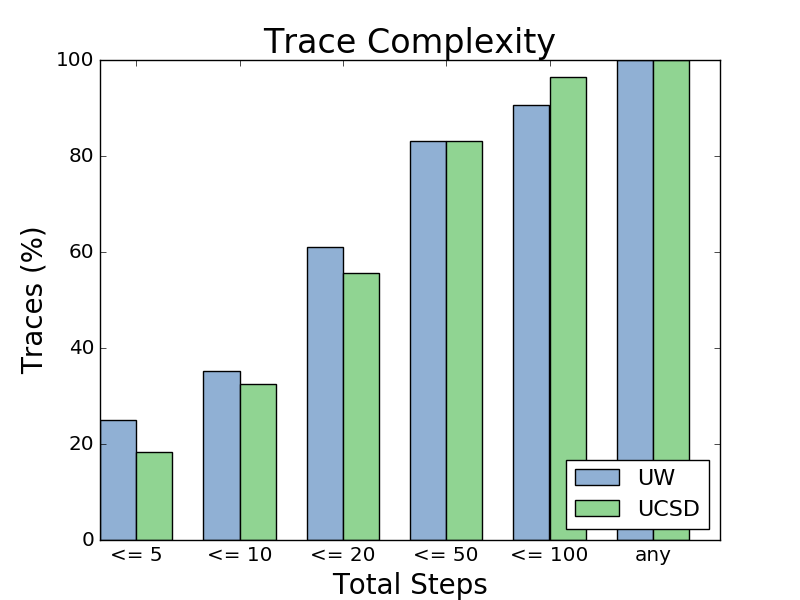
\includegraphics[width=0.7\linewidth]{trace_size_step.png}
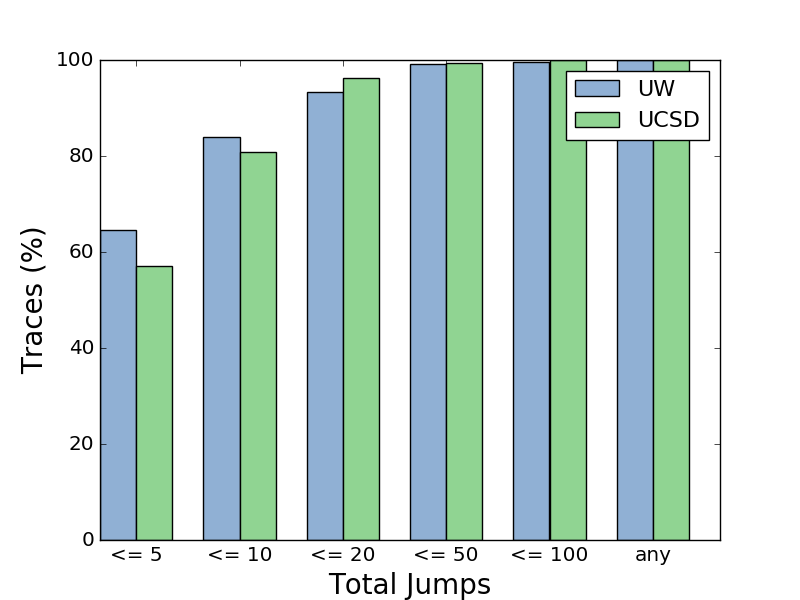
\includegraphics[width=0.7\linewidth]{trace_size_jump.png}
% \end{minipage}
% }
% \vspace{3ex}
\caption{Complexity of the generated traces. Over 80\% of the combined traces
  have a jump complexity of at most 10, with an average complexity of 7
  and a median of 5.}
\label{fig:results-complexity}
\end{figure}
%
\paragraph{Results}
\label{sec:results-complexity}
The results of the experiment are summarized in
Figure~\ref{fig:results-complexity}.
%
The average number of single-step reductions per trace is 30 for the
\ucsdbench\ dataset (45 for the \uwbench\ dataset) with a maximum of
2,745 (\resp 982) and a median of 14.5 (\resp 14.5).
%
The average number of jumps per trace is 7 (\resp 10) with a
maximium of 353 (\resp 221) and a median of 4 (\resp 4).
%
In both datasets 60\% of traces have at most 5 jumps, and 80\% or more
have at most 10 jumps.


\subsection{Qualitative Evaluation of Witness Utility}\label{sec:advantage-traces}

Next, we present a \emph{qualitative} evaluation that compares
the explanations provided by \toolname's dynamic witnesses with
the static reports produced by the \ocaml\ compiler and \sherrloc,
a state-of-the-art fault localization approach~\cite{Zhang2014-lv}.
%
In particular, we illustrate, using a series of examples drawn
from student programs in the \ucsdbench\ dataset, how \toolname's
jump-compressed traces can get to the heart of the error. Our approach
%
highlights the conflicting values that cause the program to get
stuck, rather that blaming a single one,
%
shows the steps necessary to reach the stuck state, and
%
does not assume that a function is correct just because it type-checks.
%
For each example we will present:
(1)~the code;
(2)~the error message returned \ocaml;
(3)~the error locations returned by \hlOcaml{\ocaml} and \hlSherrloc{\sherrloc};
and (4)~\toolname's jump-compressed trace.

% \begin{figure*}[ht]
% \centering
% \begin{minipage}{0.49\linewidth}
% \centering

% \begin{figure*}[htp]
%   \centering
%   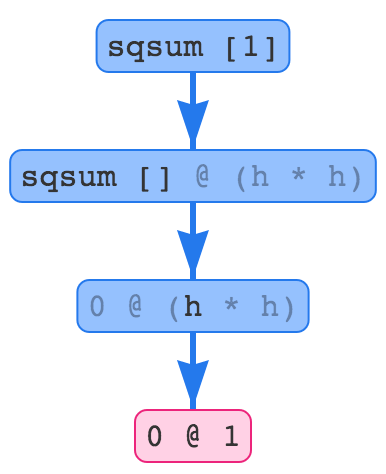
\includegraphics[height=125px]{sqsum.png}
%   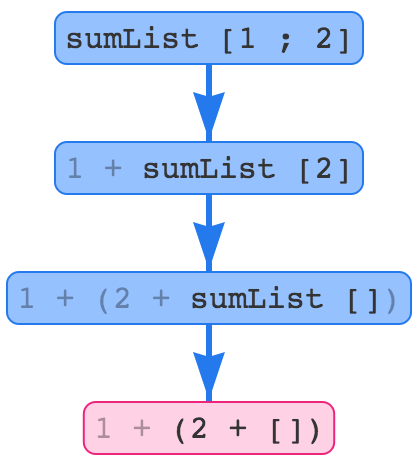
\includegraphics[height=125px]{sumlist.png}
%   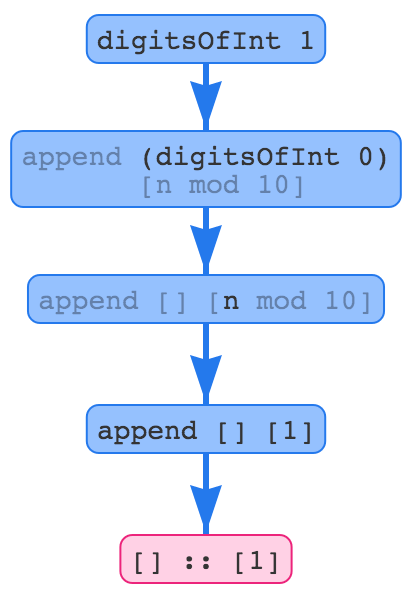
\includegraphics[height=150px]{digitsOfInt.png}
%   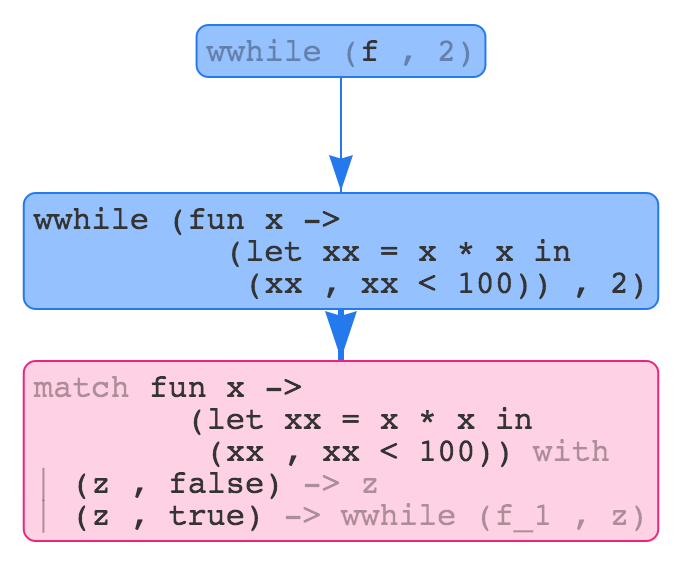
\includegraphics[height=125px]{wwhile.png}
%   \caption{(Left to right) Jump-compressed traces showing how
%     \texttt{sqsum}, \texttt{sumList}, \texttt{digitsOfInt}, and
%     \texttt{wwhile} go wrong in \S~\ref{sec:advantage-traces}.}
%   \label{fig:traces}
% \end{figure*}

\paragraph{Example: Recursion with Bad Operator}
The recursive function @sqsum@ should square each
element of the input list and then compute the sum
of the result.
%
\begin{ecode}
  let rec sqsum xs = match xs with
    | [] -> 0
    | h::t -> (*@\hlOcaml{\hlSherrloc{sqsum t}}@*) @ (h * h)
\end{ecode}
%
Unfortunately the student has used the list-append
operator |@| instead of \texttt{+}. % to compute the sum.
%
Both \ocaml\ and \sherrloc\ blame the \emph{wrong location},
the recursive call @sqsum t@, with the message
%
\begin{verbatim}
  This expression has type
    int
  but an expression was expected of type
    'a list
\end{verbatim}
%
\toolname\ produces a trace showing how the evaluation of
@sqsum [1]@ gets stuck.
%
\begin{center}
  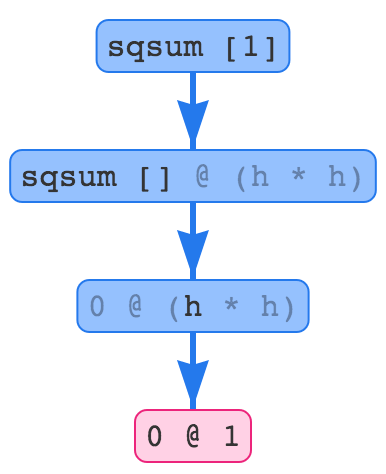
\includegraphics[height=125px]{sqsum.png}
\end{center}
%
The trace highlights the entire stuck term
(not just the recursive call), emphasizing
the \emph{conflict} between @int@ and @list@
rather than assuming one or the other is correct.

\paragraph{Example: Recursion with Bad Base Case}
%
The function @sumList@ should add up
the elements of its input list.
%
\begin{ecode}
  let rec sumList xs = match xs with
    | []    -> (*@\hlSherrloc{[]}@*)
    | y::ys -> y + (*@\hlOcaml{sumList ys}@*)
\end{ecode}
%
Unfortunately, in the base case, it returns @[]@
instead of @0@.
%
\sherrloc\ blames the base case, and \ocaml\
assumes the base case is correct and blames
the \emph{recursive call} on line 3:
%
\begin{verbatim}
  This expression has type
    'a list
  but an expression was expected of type
    int
\end{verbatim}
%
Both of the above are parts of the full story, which
is summarized by \toolname's trace showing
how @sumList [1; 2]@ gets stuck at @2 + []@.
%
\begin{center}
  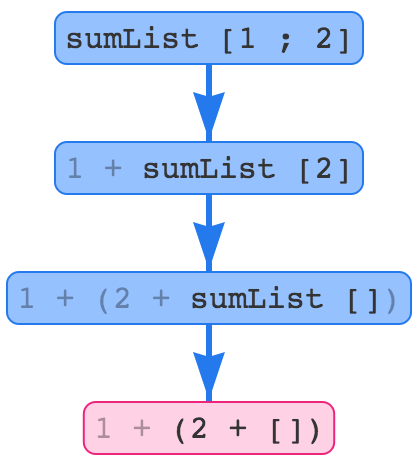
\includegraphics[height=125px]{sumlist.png}
\end{center}
%
The trace clarifies (via the third step)
that the @[]@ results from the recursive call
\hbox{@sumList []@,} and shows how it is incompatible with
the subsequent \texttt{+} operation.

%% ES: append is actually a bit problematic as we don't find the nice
%% append [1] [2] witness. instead we could find something like
%% append [_] [], but it's not as clear IMO
% Our next example is the @append@ function, which should concatenate the
% two input lists.
% %
% \begin{ecode}
% let append xs ys = match xs with
%   | []   -> ys
%   | h::t -> h :: __t__ :: ys
% \end{ecode}
% %
% The student has forgotten to make a recursive call to @append@, and
% instead tries to cons the tail @t@ directly onto the second list @ys@.
% Consing @h@ back onto the result causes \ocaml to attempt to construct
% the infinite type @'a = 'a list@, triggering an \emph{occurs-check}
% error.
% %
% \begin{verbatim}
% Error: This expression has type
%          'a list
%        but an expression was expected of type
%          'a
%        The type variable 'a occurs inside 'a list
% \end{verbatim}
% %
% %
% \begin{center}
%   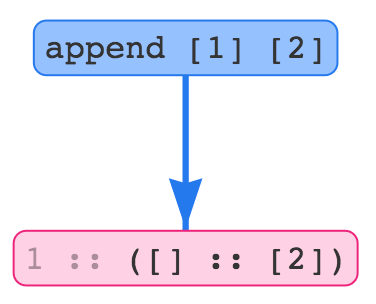
\includegraphics[height=75px]{append.png}
% \end{center}

%\pagebreak
\paragraph{Example: Bad Helper Function that Type-Checks}
%
The function @digitsOfInt@ should return a list of
the digits of the input integer.
%
\begin{ecode}
  let append x xs =
    match xs with
    | [] -> [x]
    | _  -> x :: xs

  let rec digitsOfInt n =
    if n <= 0 then
      []
    else
      append ((*@\hlSherrloc{digitsOfInt (n / 10)}@*)) [(*@\hlOcaml{n mod 10}@*)]
\end{ecode}
%
%\pagebreak
Unfortunately, the student's @append@ function \emph{conses} an element
onto a list instead of appending two lists.
%
Though incorrect, @append@ still type-checks and thus \ocaml and
\sherrloc blame the \emph{use-site} on line 10.
%
\begin{verbatim}
  This expression has type
    int
  but an expression was expected of type
    'a list
\end{verbatim}
%
In contrast, \toolname makes no assumptions about @append@,
yielding a trace that illustrates the error on line 4, by
highlighting the conflict in consing a list onto a list of integers.
%
\begin{center}
  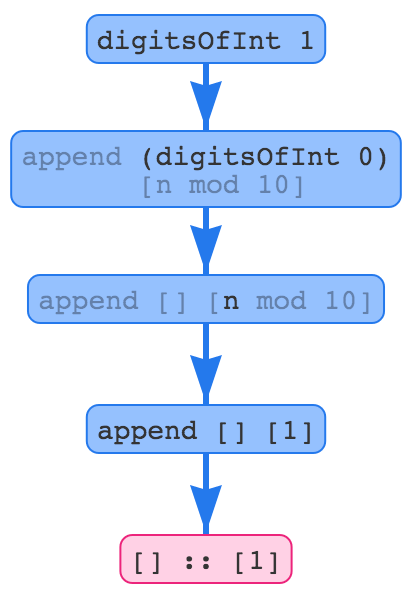
\includegraphics[height=160px]{digitsOfInt.png}
\end{center}
%

\paragraph{Example: Higher-Order Functions}
%
The higher-order function @wwhile@ is supposed
to emulate a traditional while-loop. It takes
a function @f@ and repeatedly calls @f@ on the
first element of its output pair, starting with
the initial @b@, till the second element is @false@.
%
\begin{ecode}
  let rec wwhile (f,b) =
    match f with
    | (z, false) -> z
    | (z, true)  -> wwhile (f, z)

  let f x =
    let xx = x * x in
    (xx, (xx < 100))

  let _ = wwhile ((*@\hlOcaml{\hlSherrloc{f}}@*), 2)
\end{ecode}
%
The student has forgotten to \emph{apply} @f@ at all on line 2,
and just matches it directly against a pair.
This faulty @wwhile@ definition nevertheless typechecks,
and is assumed to be correct by both \ocaml\ and \sherrloc\
which blame the use-site on line 10.
%
\begin{verbatim}
  This expression has type
    int -> int * bool
  but an expression was expected of type
    'a * bool
\end{verbatim}
%
\toolname\ synthesizes a trace that draws the eye to the
true error: the @match@ expression on line 2, and highlights
the conflict in matching a function against a pair pattern.
%
\begin{center}
  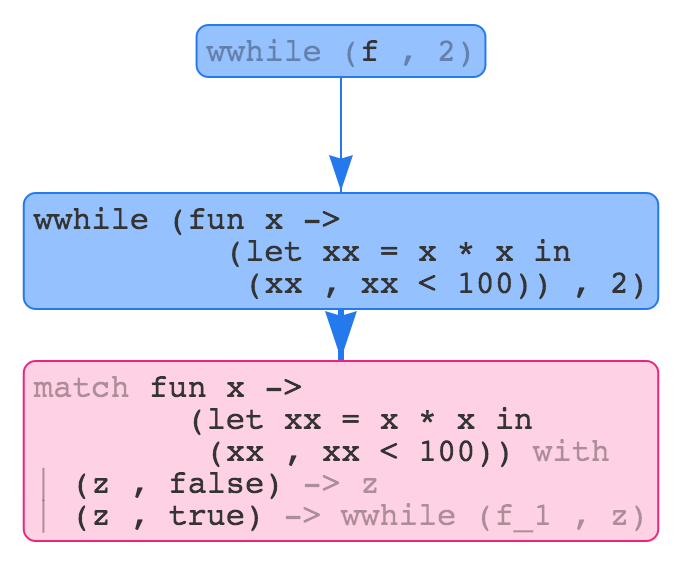
\includegraphics[height=135px]{wwhile.png}
\end{center}
%
By highlighting conflicting values, \ie\ the source and sink
of the problem, and not making assumption about function correctness, \toolname\
focusses the user's attention on the piece of code that is
actually relevant to the error.

\subsection{Quantitative Evaluation of Witness Utility}
\label{sec:user-study}
% Finally, to test the explanatory power of our jump-compressed traces, we
% ran a user study (IRB \#2014009900) at the University of Virginia (UVA).
% %
% We included four problems in an exam in the Spring session of UVA's
% undergraduate Programming Languages course (CS 4501).
% %
% We presented the 60 students in the course with ill-typed \ocaml\
% programs and asked them to
% %
% (1) \emph{explain} the type error, and
% %
% (2) \emph{fix} the type error.
% %
% For each problem the student was given the ill-typed program and
% either \ocaml's error message or \toolname's jump-compressed trace.
%
We assigned four problems to the 60 students in the course: the
@sumList@, \hbox{@digitsOfInt@,} and @wwhile@ programs from
\S~\ref{sec:advantage-traces}, as well as the following @append@ program
%
\begin{ecode}
  let append x l =
    match x with
    | []   -> l
    | h::t -> h :: t :: l
\end{ecode}
%
which triggers an occurs-check error on line 4.
%
For each problem the students were given the ill-typed program and
either \ocaml's error or \toolname's jump-compressed trace;
the full user study is available in \S~\ref{sec:user-study}.
%
Due to the nature of an in-class exam, not every student answered every
question; we received between 13 and 28 (out of a possible 30) responses
for each problem-tool pair.

We then instructed four annotators (one of whom is an author, the other
three are teaching assistants at UCSD) to classify the answers as
correct or incorrect.
%
We performed an inter-rater reliability (IRR) analysis to determine the
degree to which the annotators consistently graded the exams.
%
As we had more than two annotators assigning nominal (``correct'' or
``incorrect'') ratings we used Fleiss' kappa~\cite{Fleiss1971-du} to
measure IRR.\@
%
Fleiss' kappa is measured on a scale from $1$, indicating total
agreement, to $-1$, indicating total disagreement, with $0$ indicating
random agreement.

Finally, we used a one-sided Mann-Whitney $U$ test~\cite{Mann1947-fd} to
determine the significance of our results.
%
The null hypothesis was that the responses from students given
\toolname's witnesses were drawn from the same distribution as those
given \ocaml's errors, \ie \toolname had no effect.
%
Since we used a one-sided test, the alternative to the null hypothesis
is that \toolname had a \emph{positive} effect on the responses.
%
We reject the null hypothesis in favor of the alternative if the test
produces a significance level $p < 0.05$, a standard threshold for
determining statistical significance.

\paragraph{Threats to Validity}
Measuring understanding is a difficult task; the following summarize
the threats to the validity of our results.

\subparagraph{Construct.}
%
We used the correctness of the student's explanation of, and fix for,
the type error as a proxy for her understanding, but it is possible
that other metrics would produce different results.

\subparagraph{Internal.}
%
We assigned students randomly to two groups. The first was given
\ocaml's errors for @append@ and \hbox{@digitsOfInt@,} and \toolname's trace
for @sumList@ and \hbox{@wwhile@;} the second was given the opposite
assignment of errors and traces. This assignment ensured that: (1) each
student was given \ocaml and \toolname problems; and (2) each student
was given an ``easy'' and ``hard'' problem for both \ocaml and
\toolname. Students without sufficient knowledge of \ocaml could affect
the results, as could the time-constrained nature of an exam. For these
reasons we excluded any answers left blank from our analysis.

\subparagraph{External.}
%
Our experiment used students in the process of learning \ocaml,
and thus may not generalize to all developers. The four
programs were chosen manually, via a random selection and
filtering of the programs in the \ucsdbench dataset. In some cases we made
minor simplifying edits (\eg alpha-renaming, dead-code removal) to the
programs to make them more understandable in the short timeframe of an
exam; however, we never altered the resulting type-error. A different
selection of programs may lead to different results.

\subparagraph{Conclusion.}
%
We collected exams from 60 students, though due to the nature of the
study not every student completed every problem.
%
The number of complete submissions ranges from 13 (for the \toolname
version of @wwhile@) to 28 (for the \ocaml version of @sumList@), out of
a maximum of 30 per program-tool pair.
%
Our results are statistically significant in only 2 out of 8 tests; however,
collecting more responses per test pair was not possible as it
would require having students answer the same problem twice (once with
\ocaml and once with \toolname).

\begin{figure}[t]
% \centerline{
% \begin{minipage}{1.2\textwidth}
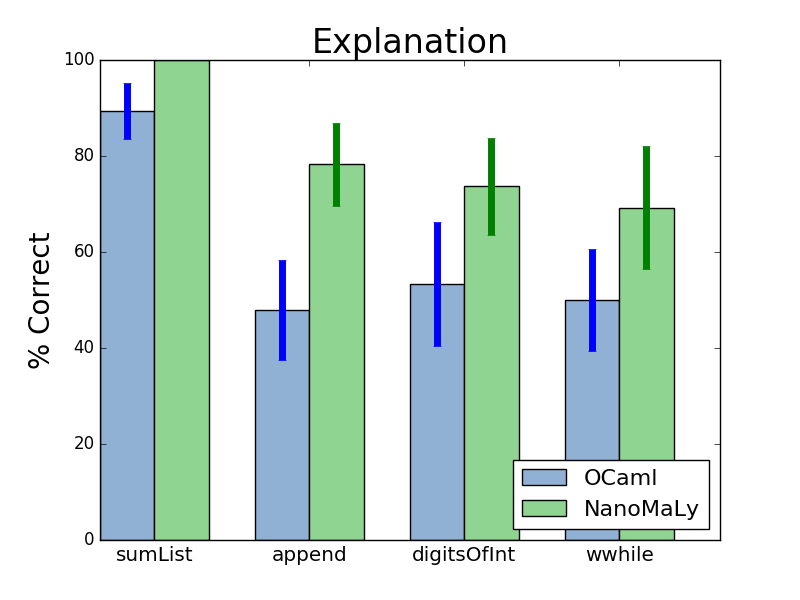
\includegraphics[width=0.7\linewidth]{user-study-reason.png}
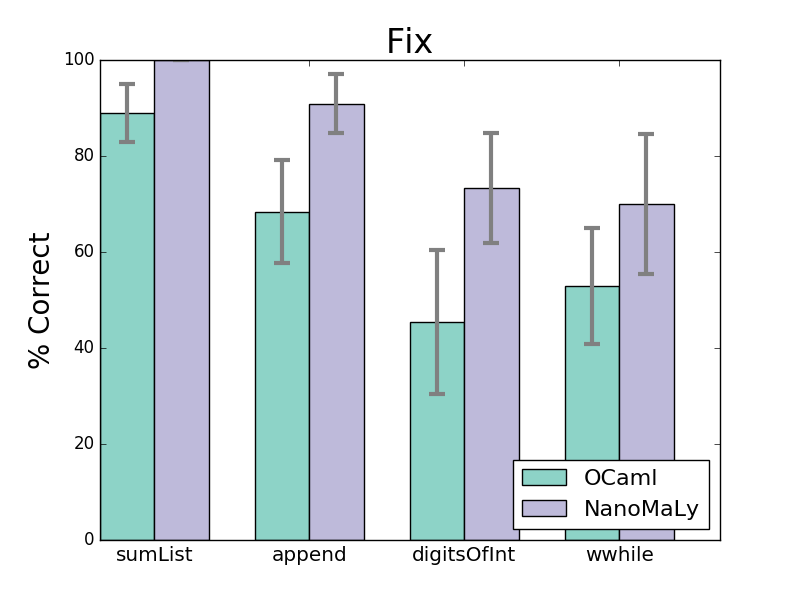
\includegraphics[width=0.7\linewidth]{user-study-fix.png}
% \end{minipage}
% }
% \vspace{3ex}
\caption{A classification of students' explanations and fixes for type
  errors, given either \ocaml's error message or \toolname's
  jump-compressed trace. The students given \toolname's jump-compressed
  trace consistently scored better ($\ge 10\%$) than those given
  \ocaml's type error. We report the result of a one-sided Mann-Whitney
  $U$ test for statistical significance in parentheses.}
\label{fig:results-user-study}
\end{figure}

\paragraph{Results}
%
The measured kappa values were $\kappa = 0.72$ for the explanations and
$\kappa = 0.83$ for the fixes; while there is no formal notion for what
consititutes strong agreement~\cite{Krippendorff2012-wd}, kappa values
above $0.60$ are often called ``substantial''
agreement~\cite{Landis1977-ey}.
%
Figure~\ref{fig:results-user-study} summarizes a single annotator's
results, which show that students given \toolname's jump-compressed
trace were consistently more likely to correctly explain
and fix the type error than those given \ocaml's error message.
%
Across each problem the \toolname responses were marked correct
$10-30\%$ more often than the \ocaml responses, which suggests that
the students who had access to \toolname's traces had a better
understanding of the type errors;
%
however, only the @append@ tests were statistically significant at
$p < 0.05$.
%


\subsection{Locating Errors with Witnesses}
\label{sec:locating}

We have seen that \toolname can effectively synthesize witnesses to
explain the majority of (novice) type errors, but a good error report
should also help \emph{locate} the source of the error.
%
Thus, our final experiment seeks to use \toolname's witnesses as
localizations.


As discussed in \S~\ref{sec:methodology}, we recorded
each interaction of our students with the \ocaml top-level system.
%
In addition to collecting ill-typed programs, we collected
subsequent, fixed versions of the programs.
%
For each ill-typed program in a student's interaction trace, we identify
the student's fix by searching for the first type-correct program
that follows it in the trace.
%
We then use an expression-level \emph{diff}~\cite{Lempsink2009-xf} to
determine which sub-expressions changed between the ill-typed program
and the student's fix, and treat those expressions as the source of the
type error.

Not all ill-typed programs will have an associated fix; furthermore,
at some point a ``fix'' becomes a ``rewrite''.
%
We do not wish to consider the ``rewrites'', so we discard outliers
where the fraction of expressions that have changed is more than one
standard deviation above the mean, establishing a diff threshold of
45\%.
%
This accounts for roughly 14\% of programs pairs we discovered, leaving
us with 2,425 program pairs.

For each pair of an ill-typed program and its fix, we run \toolname and
collect two sets of source locations:
%
(1) the source location corresponding to the stuck term; and
%
(2) the source locations that \emph{produced} the values inside the
stuck term.
%
Intuitively, these two classes of locations correspond to \emph{sinks}
and \emph{sources} for typing constraints.
%
For example, in the @sqsum@ program from \S~\ref{sec:advantage-traces}
the stuck term is \verb!0 @ 1!.
%
This corresponds to the call to \verb!@! on line 3, and contains
the literal @0@ from line 2 and the value @1@ produced by the
@*@ on line 3.

We compare \toolname's witness-based predictions against a baseline of
the \ocaml compiler as well as the state-of-the-art %type error
localization tools \sherrloc and \mycroft.
%
\sherrloc~\cite{Zhang2014-lv} attempts to predict the most likely source
of a type error by searching the typing constraint graph for constraints
that participate in many unsatisfiable paths and few satisfiable paths.
%
\mycroft~\cite{Loncaric2016-uk} reduces the localization problem to
MaxSAT by searching for a minimal subset of constraints that can be
removed, such that the resulting system is satisfiable.
%
Both tools produce a \emph{set} of equally-likely expressions to blame
for the error (in practice the set contains only a few expressions),
similar to \toolname's witness-based predictions.

We evaluate each tool based on whether \emph{any} of its predictions
identifies a changed expression.
%
There were a number of student programs where \mycroft or \sherrloc
encountered an unsupported language feature or timed out after one
minute, or where \toolname failed to produce a witness.
%
We discard all such programs in our evaluation to level the playing
field, around 15\% for each tool, leaving us with a benchmark set of
1,569 programs.

\ES{TODO: threats to validity}

\begin{figure}[t]
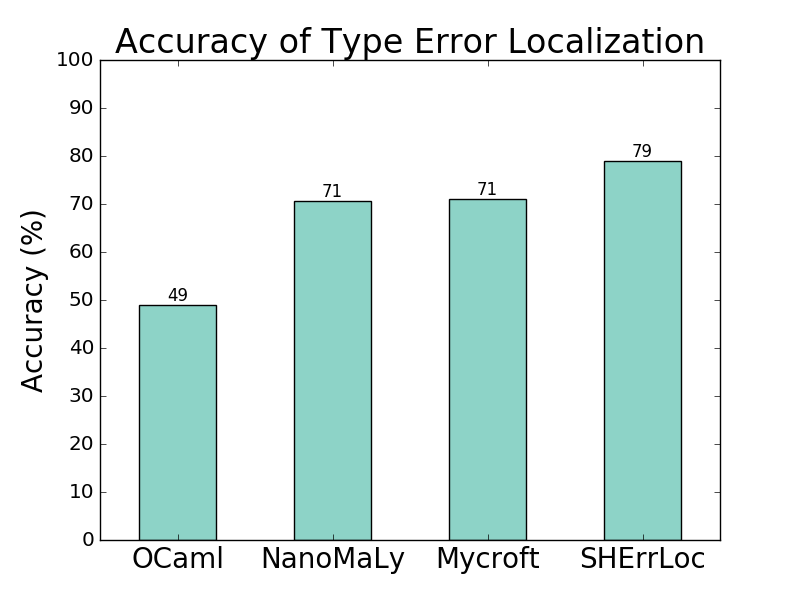
\includegraphics[width=0.7\linewidth]{blame.png}
\caption{Accuracy of type error localization. \toolname's witness-based
  predictions outperform \ocaml by 22 points, and are competitive
  with the state-of-the-art tools \mycroft and \sherrloc.}
\label{fig:results-blame}
\end{figure}

\paragraph{Results}
Figure~\ref{fig:results-blame} summarizes our results, which show that
\toolname's witnesses are competitive with \mycroft and \sherrloc in
automatically locating the source of a type error.
%
\toolname, \mycroft, and \sherrloc all outperform the \ocaml compiler,
which is not surprising given that they can produce multiple possible
error locations, while the \ocaml compiler is limited to one predicted
error location.
%
Interestingly, while all tools have a median of 2 predicted error
locations per program, \mycroft and \sherrloc have a long tail with a
maximum of 22 (\resp 12) locations, while \toolname's maximum is 5
locations.
%
We also note that while \mycroft and \sherrloc were designed
specifically to \emph{localize} type errors, \toolname's foremost
purpose is to \emph{explain} them, we consider its ability to localize
type errors an added benefit.

%%% Local Variables:
%%% mode: latex
%%% TeX-master: "main"
%%% End:


\subsection{Discussion}
\label{sec:discussion}

To summarize, our experiments demonstrate that \nanomaly finds witnesses
to type errors:
%
(1) with high coverage in a timespan amenable to compile-time analysis;
%
(2) with traces that have a low median complexity of 5 jumps;
%
(3) that are more helpful to novice programmers than traditional type
error messages; and
%
(4) that can be used to automatically locate the source of a type error.

There are, of course, drawbacks to our approach. Four that stand out
are:
%
(1) coverage limits due to random generation;
%
(2) dealing with explosions in the size of generated traces;
%
%(3) the inability to handle certain instances of infinite types; and
(3) our use of a non-parametric function type; and
%
(4) handling ad-hoc polymorphism.

\paragraph{Random Generation}
Random test generation has difficulty generating highly constrained
values, \eg\ red-black trees or a pair of equal integers. If the type
error is hidden behind a complex branch condition \nanomaly\ may not be
able to trigger it. Exhaustive testing and dynamic-symbolic execution
can address this short-coming by performing an exhaustive search for
inputs (\emph{resp}.\ paths through the program). As our experiments
show, however, novice programs do not appear to require more advanced
search techniques, likely because they tend to be simple.

% \paragraph{Infinite Types}
% Our implementation does check for infinite types inside \forcesym, but
% there are some degenerate cases where it is unable to detect
% them. Consider the following buggy @replicate@.
% %
% \begin{code}
%   let rec replicate n x =
%     if n <= 0 then
%       []
%     else
%       replicate (n-1) [x]
% \end{code}
% %
% This code produces a nested list (with @n@ levels of nesting) containing
% a single copy of @x@, instead of a list with @n@ copies of @x@. \ocaml\
% detects a cyclic \hbox{@'a = 'a list@} constraint in the recursive call
% and throws a type error, whereas \nanomaly\ happily recurses @n@ times to
% produces the nested list.  Strictly speaking, this function itself cannot
% ``go wrong'', the program would not get stuck until a \emph{client}
% attempted to use the result expecting a flat list. But this is not very
% satisfying as @replicate@ is clearly to blame. Furthermore, in our
% experience, infinite-type errors are often difficult to %some of the more difficult ones to
% debug (and to explain to novices), so better support for this scenario
% would be useful.

\paragraph{Trace Explosion}
Though the average complexity of our generated traces is low in terms of
jumps, there are some extreme outliers.
%
We cannot reasonably expect a novice user to explore a trace containing
50+ terms and draw a conclusion about which pieces contributed to the
bug in their program.
%
Enhancing our visualization to slice out program paths relevant to
specific values~\cite{Perera2012-dy}, would likely help alleviate this
issue, allowing users to highlight a confusing value and ask: ``Where
did this come from?''

\paragraph{Non-Parametric Function Type}
As we discussed in \S~\ref{sec:how-safe} some ill-typed programs
lack a witness in our semantics due to our use of a non-parametric
type $\tfun$ for functions.
%
These programs cannot ``go wrong'', strictly speaking, but would be very
difficult to \emph{use} in practice.
%
We also note that many of these programs induce cyclic typing constraints,
causing infinite-type errors, which in our experience can be particularly
difficult to debug (and to explain to novices).
%
Better support for these programs would be welcome.
%
For example, we might track how the types of inputs change between
recursive calls.
%
If we cannot find a traditional witness, we could then produce a trace
expanded to show these particular steps.

\paragraph{Ad-Hoc Polymorphism}
% Our approach can only support ad-hoc polymorphism (\eg\ type-classes in
% \haskell\ or polymorphic comparison functions in \ocaml) in limited cases
% where we have enough typing information at the call-site to resolve the
% overloading. For example, consider the @n <= 0@ test in our @fac@ example.
% @<=@ is polymorphic in \ocaml, but in this case we can make progress because
% the literal @0@ is not. If we parameterized @fac@ by a lower bound, \eg
% %
% \begin{code}
%   let rec fac n m =
%     if n <= m then
%       1
%     else
%       n * fac (n - 1) m
% \end{code}
% %
% and called @fac@ with two holes, we would get stuck at the @n <= m@
% test; not because of a type error, but because all we know about
% @n@ and @m@ at that point is that they must have the same (unknown)
% type.

Also discussed in \S~\ref{sec:how-safe}, our approach can only support
ad-hoc polymorphism (\eg\ type-classes in \haskell\ or polymorphic
comparison functions in \ocaml) in limited cases where we have enough
typing information at the call-site to resolve the overloading. This
issue is uncommon in \ocaml\ (we detected it in around 5\% of our
benchmarks), but it would surely be exacerbated by a language like
\haskell, which makes heavy use of overloading. We suspect that either
dynamic-symbolic execution or speculative instantiation of holes would
allow us to handle ad-hoc polymorphism, but defer a proper treatment to
future work.

% \begin{itemize}
% \item benchmarks: our data + seminal data
% \item both cases: \textbf{random} search sufficient to trigger runtime crash in 80\% of programs
% \item how many of the ``safe'' programs are actually safe??
% \end{itemize}

%%% Local Variables:
%%% mode: latex
%%% TeX-master: "main"
%%% End:
%!TEX root = main.tex
